%!TEX root = skripsi.tex
%-----------------------------------------------------------------------------%
\chapter{\babDua}
%-----------------------------------------------------------------------------%
Pada bab ini, dijelaskan mengenai studi literatur yang dilakukan. Studi literatur yang dilakukan digunakan sebagai dasar konsep dan teknik penelitian. Dipaparkan pula berbagai istilah, metode, dan teknik yang digunakan dalam penelitian.

%
%-----------------------------------------------------------------------------%
\section{Leksikal Semantik}
%-----------------------------------------------------------------------------%
Dalam \textit{natural language processing} (NLP), terdapat beberapa tingkatan untuk merepresentasikan suatu informasi yaitu kata, sintak, dan semantik. Kata adalah kumpulan simbol yang memiliki arti (\textit{sense}) tertentu. Bentuk kata dasar yang umumnya disimpan sebagai suatu \textit{entry} dalam kamus disebut lema. Sintak berarti struktur dari kata yang bila digabung akan membentuk arti baru. Semenatara semantik berarti arti atau makna dari kata itu sendiri. Suatu kata tidak hanya mengandung makna namun juga relasi antar kata serta struktur internal. Leksikal semantik mempelajari arti semantik, sistematik struktur, serta relasi semantik sebuah kata \citep{jurafsky2000speech}. % TODO: ask this. Too faguee

Lexeme adalah representasi abstrak dari sebuah kata dalam bentuk ortografi yang menyimpan kelas kata dan arti di dalamnya. Lexeme berukuran berhingga tersimpan dalam leksikon atau dapat juga dikenal sebagai kamus. Bahasa Inggris memiliki kamus digital yang menyimpan segala informasi mengenai kata, arti, dan strukturnya yang disebut WordNet\footnote{WordNet.princeton.edu}. WordNet tersebut sering digunakan untuk menunjang berbagai penelitian dalam bidang NLP. 

%-----------------------------------------------------------------------------%
\subsection{Word Features}
%-----------------------------------------------------------------------------%
Suatu kata dapat dilihat dari berbagai bentuk, seperti bentuk ortografi, morfologi, maupun fonemik. Suatu kata juga memiliki arti (\textit{sense}) yang merepresentasikan deskripsi terhadap kata tersebut. Sayangnya, tidak semua bentuk kata dapat dikenali oleh mesin atau digunakan untuk proses komputasi. Melalui berbagai penelitian yang telah dilakukan sebelumnya, kata dapat direpresentasikan ke dalam bentuk yang dapat dibaca oleh mesin. Berikut adalah beberapa perbandingan bentuk representasi kata yang bisa dibaca oleh manusia dan mesin.

%-----------------------------------------------------------------------------%
\subsubsection{Ortografi}
%-----------------------------------------------------------------------------%
Ortografi adalah bentuk paling dasar dari suatu kata. Bentuk ini merepresentasikan rangkaian simbol-simbol yang tersusun membentuk kata yang memiliki arti. Studi mengenai bentuk ini banyak digunakan untuk mengetahui perbandingan ejaan suatu kata. Bentuk dasar kata dapat berubah jika diberi imbuhan di mana hal tersebut dipelajari dalam bidang morfologi kata. Bentuk lain dari kata adalah bentuk fonemik yang melihat bagaimana kata tersebut dilafakan. Karena penelitian ini hanya berfokus pada teks dokumen, maka hanya diperhatikan bentuk ortografi suatu kata. Walaupun bentuk ortografi kata masih dapat dikatakan sulit digunakan untuk proses komputasi, informasi mengenai bentuk tersebut tetap perlu disimpan.

%-----------------------------------------------------------------------------%
\subsubsection{Sense}
%-----------------------------------------------------------------------------%
Sense adalah makna atau arti dari sebuah kata. Informasi mengenai makna kata dapat ditemukan dalam kamus (lexicon) bahasa yang bersangkatan. Dalam kamus, kata memiliki arti (\textit{sense}) tersendiri. Informasi mengenai \textit{sense} suatu kata penting karena bentuk kata tidak cukup untuk menggambarkan semantik kata tersebut. Suatu kata yang bentuknya sama dapat memiliki lebih dari satu \textit{sense}. Kata-kata tersebut biasa dikenal dengan istilah polisemi. Sebagai contoh kata `halaman' yang dapat berarti pekarangan rumah atau lembaran buku. Sementara adapula kasus di mana kata yang bentuknya berbeda namun memiliki arti yang sama, seperti kata `melukis' dan `menggambar'.

%-----------------------------------------------------------------------------%
\subsubsection{Word Embedding}
%-----------------------------------------------------------------------------%
Penelitian ini akan menghasilkan sebuah pasangan kata. Dari pasangan kata tersebut ingin diketahui apakah kedua kata benar berelasi hipernim-hiponim. Sangat sulit bagi mesin untuk mengetahuinya jika hanya bergantung pada bentuk asli kata tersebut. Kata perlu direpresentasikan ke dalam bentuk yang dapat dibaca oleh mesin seperti vektor sehingga dapat dihitung kemiripannya. Mengetahui hal tersebut, digunakan pemodelan \textit{word embedding} untuk mendapatkan representasi kata yang diinginkan. \textit{Word Embedding} atau juga dikenal sebagai \textit{distributed representation} adalah salah satu jenis representasi kata dalam bentuk vektor berdasarkan fitur yang dimiliki oleh kata tersebut. 

Pada tahun 2013, diperkenalkan suatu teknik pembentukan \textit{word embedding} menggunakan korpus teks berukuran besar yaitu Word2Vec \cite{mikolov2013distributed}. Terdapat dua jenis arsitektur dalam sistem tersebut yaitu model \textit{continuous skipgram} (Skipgram) dan \textit{continous bag-of-word} (CBoW). Kedua pemodelan menggunakan pembelajaran \textit{neural network} sederhana terhadap korpus yang diberikan. Model skipgram memprediksi kata-kata disekitar kata yang diberikan, sedangkan model CBoW memprediksi kata yang diberikan berdasarakan konteks disekitarnya. Implementasi teknik pemodelan tersebut telah dipublikasikan sehingga pembuatan model \textit{word embedding} dapat dilakukan dengan mudah: Word2Vec\footnote{radimrehurek.com/gensim/models/word2vec.html}.
%
% Salah satu strategi yang digunakan adalah mencari \textit{similarity} antar kata. Pencarian kemiripan antar kata dilakukan berdasarkan distribusi kata dalam kalimat atau dikatakan menggunakan teknik \textit{word embedding}.
% digunakan untuk menentukan similarity antar kata relasi yang dihasilkan dari proses \textit{Pattern Matching}. Suatu kata dapat direpresentasikan dalam bentuk vektor

%-----------------------------------------------------------------------------%
\subsubsection{POS Tagging}
%-----------------------------------------------------------------------------%
Setiap kata dalam kalimat dapat dikelompokkan berdasarkan kategori tertentu. \textit{Part-of-Speech Tagging} (POS Tagging) adalah proses pengelompokan setiap kata dalam suatu kalimat ke dalam kelas kata yang bersesuaian. Kelas kata yang umum dikenal adalah \textit{noun}, \textit{verb}, \textit{adjective}, \textit{adverb}, \textit{conjunction}, dan lainnya. Penelitian lain mengelompokkan kata berdasarkan kelas kata yang didefinisikan sendiri seperti Penn Treebank yang mengelompokkan ke dalam 45 kelas \citep{marcus1993building} dan Brown Corpus yang mengelompokkan ke dalam 87 kelas \citep{francis1979brown}. Informasi tersebut dapat digunakan untuk mendapatkan pengetahuan lebih dalam mengenai suatu kata. 

Beberapa penelitian pembangunan POS \textit{tagger} untuk Bahasa Indonesia telah dilakukan sebelumnya oleh \cite{adriani2009statistical} dan \cite{dinakaramani2014designing}. Penelitian yang dilakukan oleh \cite{adriani2009statistical} berusaha melakukan komparasi antara dua metode dalam pembangunan model POS \textit{Tagger} yang lebih baik. Sementara penelitian yang dilakukan oleh \cite{dinakaramani2014designing} lebih berfokus untuk membangun korpus yang dapat digunakan sebagai model. Penelitian tersebut menghasilkan 23 \textit{tagset} dan korpus Bahasa Indonesia yang telah di-\textit{tag} secara manual. Dari korpus tersebut, model untuk POS \textit{tagging} dapat dibangun dengan bantuan \textit{tools} Stanford POS Tagger \citep{toutanova2003feature}.

%-----------------------------------------------------------------------------%
\subsection{Relasi Kata}
%-----------------------------------------------------------------------------%
Relasi menggambarkan hubungan yang dimiliki oleh suatu hal dengan yang lain (KBBI). Dalam bidang matematika, relasi memetakan suatu anggota dari himpunan satu ke himpunan lain sesuai dengan hubungan yang didefinisikan. Dalam penelitian ini, relasi yang diperhatikan adalah relasi kata yang berarti satu kata akan dipetakan dengan kata lain. Kemudian, karena relasi yang diteliti adalah hiponim-hipernim, domain katanya adalah kata benda (\textit{noun}) dalam Bahasa Indonesia.

Satu relasi dapat terdiri dari beberapa entitas dan dituliskan dalam bentuk tuple $t = (e_1, e_2, ..., e_n)$ di mana $e_i$ adalah suatu entitas yang memiliki relasi $r$ dalam dokumen $D$ \citep{bach2007review}. Relasi sinonim dapat ditulis dalam notasi tersebut. Selain relasi yang mengandung beberapa entitasi, banyak relasi yang hanya menghubungkan antar dua entitas atau biasa disebut relasi biner. Contoh relasi biner antara dua kata adalah terletak-di(Universitas Indonesia, Depok), dibaca `Universitas Indonesia terletak di Depok', atau ditulis-oleh(Habis Gelap Terbitlah Terang, RA Kartini), dibaca `Habis Gelap Terbitlah Terang ditulis oleh RA Kartini'. Relasi kata dapat didefinisikan secara bebas seperti contoh sebelumnya maupun berdasarkan padanan tertentu seperti relasi semantik.

Semantik adalah arti (\textit{sense}) dari kata. Relasi semantik kata adalah hubungan yang dimiliki antar kata berdasarkan arti atau makna dari kata tersebut. Beberapa relasi semantik kata adalah sebagai berikut \citep{miller1995wordnet}.
\begin{itemize}
  \item Sinonim adalah relasi antara kata yang berbeda namun memiliki arti yang sama. Semua kelas kata dapat memiliki relasi sinonim. Relasi sinonim bersifat simetris yang berarti jika `sinonim($k_1$,$k_2$)' benar maka `sinonim($k_2$,$k_1$)' juga benar. Dalam WordNet, relasi ini direpresentasikan dalam bentuk \textit{synset} dan bersifat simetris. Sebagai contoh kata 'makan', 'melahap', dan 'menyantap'\footnote{bahasa.cs.ui.ac.id/iwn/WordNet.php?keyword=makan} memiliki makna yang sama.
  \item Antonim menghubungan dua kata yang memiliki arti yang saling berkebalikan. Umumnya relasi ini dimiliki oleh kata yang berada dalam kelas kata sifat (\textit{adverb}) dan kata keterangan (\textit{adjective}). Sama seperti sinonim, relasi ini memiliki sifat simetris. Sebagai contoh kata 'tinggi' memiliki makna yang berkebalikan dengan kata 'pendek'\footnote{compling.hss.ntu.edu.sg/omw/cgi-bin/wn-gridx.cgi?gridmode=wnbahasa\&synset=05097536-n\&lang=ind\&lang2=ind}.
  \item Hiponim adalah relasi yang menyatakan hubungan kata yang lebih khusus. Sementara untuk kata yang lebih umum dikenal dengan relasi hipernim. Kedua relasi ini diperuntukan kelas kata benda (\textit{noun}) dan umumnya satu kata memiliki hanya satu hipernim. Kedua relasi ini bersifat transitif, sehingga dapat digambarkan dalam bentuk hirarki. Sebagai contoh `macan', `singa', `citah', dan `jaguar' (hiponim) adalah `kucing' (hipernim)\footnote{compling.hss.ntu.edu.sg/omw/cgi-bin/wn-gridx.cgi?gridmode=wnbahasa\&synset=02127808-n\&lang=ind\&lang2=ind}. Kemudian jika diketahui `kucing' adalah hiponim dari `hewan', dapat pula dikatakan bahwa `macan', `singa', `citah', dan `jaguar' adalah `hewan'.
  \item Meronim dan holonim adalah relasi yang menyatakan hubungan bagian satu dengan yang lain, di mana meronim menyatakan subbagian dan holonim menyatakan bagian yang lebih besar. Seperti relasi hyponym-hypernym, relasi meronim-holonim bersifat transitif dan dapat digambarkan dalam bentuk hirarki. Dalam WordNet, relasi ini dibagi ke dalam tiga tipe yaitu \textit{part-meronym}, \textit{member-meronym}, dan \textit{substance-meronym}. Sebagai contoh `sel' (holonim) memiliki `nukleus', `sitoplasma', `membran', dan `vakuola' (meronim)\footnote{compling.hss.ntu.edu.sg/omw/cgi-bin/wn-gridx.cgi?usrname=\&gridmode=wnbahasa\&synset=00006484-n\&lang=ind\&lang2=ind}. 
  \item \textit{Troponymy} adalah relasi seperti hiponim-hipernim yang khusus untuk kelas kata kerja (\textit{verb}). Dalam Bahasa Inggris, contoh kata yang memiliki relasi ini adalah 'march' dan 'walk'.
\end{itemize}

Relasi semantik hiponim-hipernim memiliki dua tipe yang lebih spesifik yaitu relasi hiponim-hipernim antar \textit{class} dan relasi hipernim-hiponim antar \textit{instance} dan \textit{class}. Suatu kata disebut sebagai \textit{instance} atau entitas jika wujudnya dapat tergambarkan dengan jelas walaupun tidak harus berbentuk fisik. Sementara \textit{class} atau biasa disebut konsep adalah abstraksi dari suatu kategori yang mengandung sejumlah objek dengan ciri-ciri yang sama. Sebagai contoh pasangan kata relasi hipernim-hiponim antar \textit{class} adalah hiponim(sarapan, makanan), dibaca `sarapan adalah hiponim dari makanan'. Sementara pasangan kata relasi hipernim-hiponim antar \textit{instance} dan \textit{class} adalah hiponim(Chairil Anwar, penulis).


%-----------------------------------------------------------------------------%
\section{Resource Leksikal Semantik}
%-----------------------------------------------------------------------------%
Leksikal semantik \textit{resource} adalah suatu korpus yang menyimpan informasi mengenai kata, makna kata, serta relasi antar kata. Leksikal semantik \textit{resource} yang terkenal di antaranya adalah kamus, tesaurus, ensiklopedia, dan WordNet. Informasi tersebut juga perlu disimpan sedemikian sehingga dapat dapat dibaca mesin dan digunakan untuk proses komputasi. Bahasa Inggris sudah memiliki leksikal semantik \textit{resource} yaitu WordNet yang banyak digunakan untuk berbagai penelitian. Sementara untuk Bahasa Indonesia, penelitian yang berusaha membangun WordNet telah dilakukan sebelumnya. Sayangnya masih ditemukan beberapa kekurangan dari WordNet Bahasa Indonesia yang sudah ada. 
% TODO: tambahin disini apakek 

%-----------------------------------------------------------------------------%
\subsection{WordNet}
%-----------------------------------------------------------------------------%
WordNet adalah kamus leksikal yang tersimpan secara digital sehingga dapat digunakan untuk berbagai keperluan komputasi \citep{miller1995wordnet}. Pembuatan WordNet dilatarbelakangi keperluan mendapatkan \textit{sense} atau arti semantik suatu kata. Informasi tersebut perlu disimpan dan dapat dibaca oleh mesin. WordNet pertama dibuat oleh \cite{miller1995wordnet} berbasis Bahasa Inggris dan sekarang dikenal dengan nama Princeton WordNet\footnote{WordNet.princeton.edu} (PWN). WordNet menyimpan informasi dalam bentuk \textit{database} di mana setiap \textit{entry} adalah pasangan \textit{synset} dan arti semantiknya (\textit{sense}). Set sinonim (\textit{synset}) adalah himpunan kata yang memiliki arti yang sama atau saling berelasi \textit{synonym}. 

Kata dalam WordNet dikelompokkan ke dalam beberapa kelas kata yaitu kata benda (\textit{noun}), kata kerja (\textit{verb}), kata sifat (\textit{adjective}), dan kata keterangan (\textit{adverb}). WordNet juga menyimpan informasi mengenai relasi semantik antar \textit{synset}. Relasi yang disimpan adalah sinonim, antonim, hiponim, hipernim, meronim, holonim, \textit{troponymy}, dan \textit{entailment}. Hingga penulisan ini, versi WordNet yang sudah ada adalah versi 3.1 yang dapat diakses melalui situs resminya maupun diunduh datanya. Sementara bentuk aplikasinya yang sudah terintegrasi dengan sistem UNIX/Linux adalah versi 3.0. 

Penelitian mengenai WordNet Bahasa Indonesia pernah dilakukan sebelumnya oleh \cite{putra2008building} serta \cite{margaretha2008comparing}. Indonesian WordNet\footnote{bahasa.cs.ui.ac.id/iwn/} (IWN) dibangun menggunakan metode \textit{mapping} antara WordNet yang sudah ada ke dalam Bahasa Indonesia \citep{putra2008building}. WordNet yang digunakan sebagai dasarnya adalah Princeton WordNet. Synset dalam PWN akan dipetakan ke dalam \textit{entry} Kamus Besar Bahasa Indonesia (KBBI), sehingga menghasilkan hasil yang berkualitas baik secara cepat dan mudah. Penelitian tersebut menghasilkan 1441 \textit{synset} dan 3074 \textit{sense}. Relasi semantik antar \textit{synset} diperoleh melalui pemetaan antara \textit{synset} IWN dengan \textit{synset} PWN, sehingga relasi yang dikandung oleh PWN dapat diwarisi .

Pengembangan WordNet untuk Bahasa Indonesia juga dilakukan oleh Nanyang Technology University (NTU) sejak tahun 2011 dan diberi nama WordNet Bahasa\footnote{wn-msa.sourceforge.net/} \citep{noor2011creating}. WordNet ini telah diintegrasi dengan salah satu \textit{tools} NLP berbasis Python yaitu nltk sehingga dapat dengan mudah digunakan dalam komputasi. WordNet Bahasa juga memanfaatkan PWN untuk memperoleh relasi semantik antar \textit{synset}. Pada penelitian ini, dimanfaatkan \textit{tools} tersebut untuk membangun \textit{seed} relasi semantik antar kata dalam Bahasa Indonesia.

Walau beberapa penelitian sudah dilakukan sebelumnya, WordNet Bahasa Indonesia masih memiliki beberapa kekurangan. Jumlah kata yang terkandung di dalamnya masih terbatas. Sementara itu, relasi semantik antar kata yang dimiliki oleh WordNet Bahasa Indonesia merupakan hasil turunan dari relasi semantik WordNet Princeton. Hal ini menyebabkan ketergantungan dengan struktur dari PWN untuk mendapatkan relasi semantik suatu kata. Selain itu, beberapa kata maupun \textit{synset} Bahasa Indonesia juga tidak dapat dipetakan secara tepat ke \textit{synset} PWN yang menyebabkan adanya kata yang kehilangan arti atau mendapat arti yang kurang tepat. Jika dibentuk suatu relasi biner yang memetakan satu kata dengan kata lain berdasarakan relasi semantiknya, hasil yang didapatkan terlihat kurang baik. Untuk itu, dicetuskanlah penelitian untuk mengekstrak relasi semantik dalam Bahasa Indonesia secara mandiri. 

%-----------------------------------------------------------------------------%
\subsection{Wikipedia}
%-----------------------------------------------------------------------------%
Wikipedia\footnote{www.wikipedia.org} adalah ensiklopedia terbuka yang memuat berbagai bahasa dan merupakan hasil tulisan dari berbagai kontributor \citep{denoyer2006wikipedia}. Wikipedia adalah salah satu korpus teks dokumen terbesar yang disimpan secara \textit{online} dan dapat diakses serta diunduh secara bebas. Wikipedia dikelola oleh organisasi nonprofit bernama Wikimedia Foundation. Pada tahun 2009, jumlah kontributor Wikipedia Bahasa Indonesia mencapai 2.502 pengguna aktif. Walau ditulis oleh berbagai narasumber, artikel yang dimuat dalam Wikipedia disusun secara terstruktur dan menggunakan bahasa yang cukup formal. Wikipedia juga memuat berbagai informasi umum terbaru \citep{arnold2014extracting}.

Hingga Mei 2017, Wikipedia Bahasa Indonesia telah memuat lebih dari 400.000 artikel dari berbagai domain dan terus berkembang secara pesat. Artikel-artikel yang disimpan dalam Wikipedia dapat diunduh secara gratis dalam bentuk \textit{dumps}\footnote{dumps.wikimedia.org} dengan format XML. Beberapa tipe \textit{dump} yang dapat dipilih, diantarnya adalah halaman seluruh artikel, halaman artikel beserta \textit{revision history}, daftar judul artikel, dan lainnya. Secara berkala, Wikimedia membuat \textit{dump} terhadap seluruh artikel terakhir yang disimpan untuk setiap bahasa. Pada situs yang menyediakan pengunduhan data Wikipedia, terdapat tanggal unik yang menyatakan tanggal terakhir data tersebut di-\textit{update}.

% wikipedia sebagai lexical semantic resource
Artikel dalam Wikipedia terdiri dari berbagai domain kategori dan memuat berbagai entitas leksikal. Kata-kata tersebut dapat ditemukan dalam berbagai leksikal semantik \textit{resource} yang sudah ada. \cite{zesch2007analyzing} melakukan penelitian yang membandingkan data Wikipedia dengan leksikal semantik \textit{resource} yang sudah ada seperti kamus, tesaurus, WordNet, dan ensiklopedia. Istilah-istilah yang ada dalam Wikipedia lebih mirip dengan ensiklopedia dibanding kamus, tesaurus, maupun WordNet karena memuat lebih banyak  kata benda (\textit{noun}) dibanding kata sifat (\textit{adjective}) atau kata kerja (\textit{verb}). Selain itu, Wikipedia juga mengandung banyak kata yang merupakan \textit{named entity} atau \textit{domain specific terms}. Penelitian ini berfokus pada kata-kata yang merupakan kata benda, sehingga Wikipedia cocok digunakan. 

Walau ditulis secara kolaboratif, Wikipedia memuat artikel secara terstruktur di mana pada paragraf pertama umumnya berisi kalimat-kalimat definisi mengenai topik yang sedang dibahas. Paragraf selanjutnya memuat bahasan yang lebih rinci. Setiap artikel ditulis dalam bahasa yang formal dan terstruktur. Selain itu, sudah banyak penelitian ekstraksi relasi semantik kata beberbasis \textit{pattern} yang menggunakan artikel Wikipedia sebagai \textit{resource} seperti penelitian yang dilakukan oleh \cite{ruiz2005automatic} dan \cite{arnold2014extracting}. Melihat banyaknya manfaat dan kelebihan Wikipedia, diputuskan untuk menggunakan Wikipedia sebagai leksikal semantik \textit{resource} dalam penelitian ini. 


%-----------------------------------------------------------------------------%
\subsection{Korpus Pasangan Kata Relasi Semantik}
%-----------------------------------------------------------------------------%
Korpus adalah data yang dengan format yang dapat dibaca oleh mesin dan memiliki fungsi spesifik \citep{atkins1992corpus}. Saat ini, belum ada korpus independen yang menyimpan relasi semantik antar kata dalam Bahasa Indonesia. Relasi semantik Bahasa Indonesia yang ada saat ini didapatkan dari hasil relasi turunan pemetaan \textit{synset} Bahasa Indonesia dengan WordNet Princeton. 

Korpus relasi semantik yang ingin dibuat menyimpan informasi dalam bentuk pasangan kata berelasi serta relasi yang menghubungkannya. Pasangan kata relasi akan disebut sebuah relasi biner dengan format sebagai berikut.
\[ hiponim(w_1,w_2) \]
\noindent Format di atas dibaca $w_1$ adalah hiponim dari $w_2$ atau dapat dikatakan juga bahwa $w_2$ adalah hipernim dari $w_1$. Selanjutnya pasangan kata relasi akan disebut sebagai \textit{pair}. Pada penelitian ini, korpus pasangan kata relasi hipernim-hiponim yang dibentuk tidak memperdulikan jarak hubungan antar kata, sehingga korpus dapat mengandung \textit{pair} hiponim(kelinci,mamalia) serta hiponim(kelinci,makhluk hidup).


%-----------------------------------------------------------------------------%
\section{Relation Extraction}
%-----------------------------------------------------------------------------%
\textit{Relation extraction} adalah cabang dari \textit{Information Extraction} (IE) yang berfokus pada proses ekstraksi relasi antar kata. Proses ini berusaha mengekstrak informasi terstruktur dengan definisi yang diinginkan dari teks dokumen atau \textit{resource} yang tidak terstruktur. Beberapa contoh penelitian ini seperti \textit{named entity recognition} (NER) yang berusaha mengidentifikasi apakah suatu entitas adalah orang, organisasi, atau lokasi \citep{bikel1999algorithm}. 

%-----------------------------------------------------------------------------%
% \subsection{Semantic Relation Extraction}
% TODO: tambahin penelitian yang gak pake pattern
%-----------------------------------------------------------------------------%
\textit{Semantic relation extraction} mengkhususkan pada proses ekstraksi relasi semantik antar kata. Penelitian dalam bidang ini sudah banyak dilakukan dengan berbagai metode. Salah satu metode populer untuk mendapatkan relasi semantik kata adalah menggunakan \textit{pattern extraction} dan \textit{pattern matching} seperti yang telah dilakukan pada penelitian \cite{hearst1992automatic}, \cite{ruiz2005automatic}, dan \cite{arnold2014extracting}. Penelitian lain memanfaatkan distribusi kata untuk memperoleh \textit{semantic distance} antar kata. \textit{Semantic distance} adalah nilai yang merepresentasikan kedekatan antar kata berdasarkan semantiknya.

Penelitian yang dilakukan oleh \cite{hearst1992automatic} merupakan salah satu penelitian awal ekstraksi relasi semantik yang menggunakan metode \textit{pattern extraction} dan \textit{matching}. Hearst menggunakan \textit{lexico-syntactic pattern} untuk mendapatkan pasangan kata relasi tanpa membutuhkan pengetahuan sebelumnya dan dapat diaplikasikan dalam teks apapun. Pada awal pengembangan, Hearst mendifiniskan manual dua \textit{pattern} berdasarkan hasil observasi dari teks. Selanjutnya, \textit{pattern} baru didapat menggunakan langkah berikut. 
\begin{enumerate}
  \item Tentukan relasi yang akan diamati dan kumpulkan entitas yang menggambarkan relasi tersebut.
  \item Dalam teks dokumen, cari lokasi di mana entitas-entitas tersebut berada dan simpan kata-kata di antaranya (lingkungan).
  \item Cari kesamaan dari teks yang terekstraksi dan bentuk suatu \textit{pattern} baru.
  \item Jika \textit{pattern} baru telah terbukti benar, gunakan \textit{pattern} tersebut untuk mendapatkan entitas baru.
\end{enumerate}
Proses evaluasi dilakukan dengan membandingkan entitas yang dihasilkan dengan \textit{synset} dalam WordNet. 

Penelitian yang dilakukan oleh \cite{ruiz2005automatic}, memanfaatkan WordNet dan Wikipedia sebagai korpus untuk mendapatkan pasangan kata relasi. Penelitian ini dilakukan untuk mengekstrak kata dengan relasi hipernim-hiponim dan sinonim. Pertama dilakukan \textit{entry sense disambiguation} yang merupakan tahap \textit{pre-processing} untuk memetakan setiap \textit{entry} dalam Wikipedia dengan \textit{synset} dalam WordNet. Tahap berikutnya adalah ekstraksi \textit{pattern} antara dua kata yang bertipe konsep. Jika terdapat dua konsep yang saling berhubungan dan memiliki suatu relasi semantik dalam WordNet maka kalimat yang mengandung dua konsep tersebut akan disimpan. Proses tersebut menghasilkan daftar relasi semantik dengan masing-masing memiliki \textit{pattern} di dalamnya. Dari banyak \textit{pattern} yang dihasilkan, proses selanjutnya adalah \textit{pattern generalisation} yang bertujuan membuat pattern yang lebih umum. Tahap ini memanfaatkan algoritma \textit{edit-distance} dengan modifikasi. Setelah mendapatkan \textit{pattern}, tahapan terakhir adalah menggunakannya ke dalam korpus untuk memperoleh entitas baru.

Penelitian yang dilakukan \cite{arnold2014extracting} juga memanfaatkan korpus Wikipedia dan menggunakan metode berbasis \textit{pattern}. Selain hipernim-hiponim, penelitian ini juga mengidentifikasi relasi meronim-holonim dan sinonim. Kalimat definisi dalam artikel Wikipedia di-\textit{parse} menggunakan \textit{Finite State Machine} (FSM) dan konsep-konsep baru diekstrak menggunakan \textit{pattern} yang telah didefinisikan. Penelitian lain yang dilakukan oleh \cite{sumida2008hacking} memanfaatkan struktur hirariki internal Wikipedia dalam mengekstraksi \textit{pattern} relasi untuk Bahasa Jepang. 


%TODO PENTING BANGET: HARUS DITAMBAHIN
%-----------------------------------------------------------------------------%
\section{Pattern Analysis}
%-----------------------------------------------------------------------------%
\textit{Pattern} adalah suatu bentuk yang dapat merepresentasikan kumpulan data dengan ukuran besar. Pada teks dokumen, \textit{pattern} dapat terbentuk secara eksplisit ataupun implisit. Secara eksplisit seperti \textit{lexico-syntactic pattern} yang terbentuk dari kata-kata di dalam dokumen tersebut. Sementara \textit{pattern} terbentuk secara implisit jika dilihat dari kemiripan vektor yang merepresentasikan dokumen atau kata-kata di dalam dokumen tersebut.

\textit{Lexico-syntactic pattern} adalah \textit{pattern} yang hanya memanfatkan kata-kata dalam korpus dokumen untuk digunakan pada tahap \textit{string matching}. Salah satu \textit{pattern} leksikal yang terkenal adalah Hearst Pattern yang merepresentasikan pola-pola untuk mendapatkan relasi hiponim antar kata dalam dokumen \citep{hearst1992automatic}. Menurut Hearst, beberapa syarat yang harus dipenuhi suatu \textit{lexico-syntactic pattern} yang baik adalah sebagai berikut.
\begin{itemize}
  \item Kemunculan \textit{pattern} sering pada teks dan dalam berbagai domain sehingga dapat mengekstrak banyak entitas.
  \item Merepresentasikan relasi yang diinginkan sehingga hasil ekstraksi juga benar.
  \item Dapat dikenali tanpa membutuhkan pengetahuan sebelumnya sehingga dapat dibentuk dalam situasi apapun.
\end{itemize}

%-----------------------------------------------------------------------------%
\subsection{Textual Pattern}
%-----------------------------------------------------------------------------%
\textit{Pattern} yang dibentuk adalah \textit{pattern} tekstual yang hanya terdiri dari kata-kata. Sebuah \textit{pattern} mengandung tiga bagian penting, yaitu \textit{tag} hiponim, \textit{tag} hipernim, dan kata lainnya. \textit{Tag} hiponim-hipernim merepresentasikan letak kata yang merupakan kata hiponim-hipernim berada. Sementara kata lainnya adalah kata-kata yang harus sama saat dibandingkan dalam proses \textit{pattern matching}. Sebagai contoh terdapat tekstual \textit{pattern} `{\tagHyponym} adalah {\tagHypernym} yang'. \textit{Pattern} tersebut akan membuat kata yang terletak sebelum kata `adalah' dikenali sebagai kata hiponim. Selain itu, kata yang posisinya setelah kata `adalah' dan sebelum kata `yang' dikenali sebagai kata hipernim. Diberikan kalimat `harimau adalah kucing yang berukuran besar', maka `harimau' merupakan hiponim dan `kucing' merupakan hipernim. Di dalam kata lainnya, terdapat \textit{tag} khusus yang digunakan dalam penelitian ini yaitu {\tagStart} dan {\tagEnd}. Kedua \textit{tag} tersebut membantu mengetahui kata-kata yang terletak pada awal dan akhir kalimat.

%-----------------------------------------------------------------------------%
\subsection{Pattern Extraction}
%-----------------------------------------------------------------------------%
\textit{Pattern extraction} atau \textit{pattern recognition} adalah salah satu cabang dalam \textit{machine learning} yang berusaha mencari pola kemiripan tertentu dari kumpulan data yang diberikan. \textit{Pattern} yang akan dibentuk adalah \textit{textual pattern}, sehingga proses pembentukan \textit{pattern} dilakukan dengan cara mencari kemiripan di antara kumpulan kalimat yang jumlahnya banyak. Penelitian ini memanfaatkan struktur data \textit{tree} dalam pembentukan \textit{pattern} yang secara detil dapat dilihat pada bab \ref{sec:tree}. Suatu kalimat ditokenisasi dan \textit{sequence} kata yang dihasilkan membentuk \textit{path} dalam \textit{tree}. \textit{Node} dalam \textit{tree} merepresentasikan satu kata dalam kalimat. \textit{Sequence} kata yang sering muncul menjadi \textit{pattern} terbaik untuk kumpulan dokumen yang sedang diamati. 

%-----------------------------------------------------------------------------%
\subsection{Pattern Matching}
%-----------------------------------------------------------------------------%
\textit{Pattern matching} adalah proses untuk mencocokkan suatu \textit{pattern} terhadap kumpulan data yang belum dianotasi. Jika diberikan sebuah \textit{pattern} tekstual, proses ini akan mencocokkan \textit{sequnce} kata dalam \textit{pattern} terhadap \textit{sequence} kata dalam kalimat yang diamati. Jika terdapat satu token dalam \textit{sequence pattern} yang tidak sama dengan \textit{sequence} kalimat, maka proses pencarian dapat dikatakan gagal. Sementara, jika terdapat \textit{sequnce} kata dalam kalimat yang sama dengan \textit{sequence} kata dalam \textit{pattern}, maka dianggap berhasil dan akan menghasilkan sebuah \textit{pair} baru. Penelitian ini memanfaatkan representasi \textit{suffix tree} untuk mempermudah proses pencarian. Lebih detil mengenai proses pembentukan \textit{suffix tree} dan pencocokan \textit{pattern}, dapat dilihat pada bab \ref{sec:suffix-tree}.


%TODO PENTING BANGET: HARUS DITAMBAHIN
%-----------------------------------------------------------------------------%
\section{Tree Representation} 
%-----------------------------------------------------------------------------%
Dalam penelitian ini, segala hal yang berkaitan dengan proses pembuatan \textit{pattern} (\textit{pattern extraction}) maupun ekstraksi \textit{pair} baru (\textit{pattern matching}), memanfaatkan struktur data \textit{tree}. Struktur data tersebut mempermudah proses pembentukan maupun pencarian \textit{pattern} tekstual karena setiap kata dapat direpresentasikan sebagai \textit{node}. Proses pencocokan \textit{sequence} kata dalam dapat dengan mudah dilakukan dengan menelusuri \textit{path} dari \textit{root node} dalam \textit{tree}. Dua tipe \textit{tree} yang menjadi fokus penelitian adalah \textit{standard tree} dan \textit{suffix tree}.
% Dalam bidang bioinformatik, \textit{suquence analysis} digunakan untuk mengetahui apakah suatu DNA atau RNA mengandung \textit{sequnce} tertentu. Pada penelitian ini, \textit{pattern} yang dihasilkan adalah \textit{pattern} leksikal yang merupakan deretan kata-kata. Algoritma seperti \textit{standard tree} dan \textit{suffix tree} dimanfaatkan secara berurut untuk proses \textit{pattern extraction} dan \textit{matching}.

%-----------------------------------------------------------------------------%
\subsection{Standard Tree} \label{sec:tree}
%-----------------------------------------------------------------------------% 
\textit{Standard Tree} \citep{weiss2010data} adalah bentuk paling dasar suatu \textit{tree}. \textit{Tree} ini akan membentuk \textit{path} untuk setiap \textit{sequence string} yang menjadi masukan. \textit{Standard Tree} untuk suatu himpunan \textit{string} $S$ adalah \textit{ordered tree} dengan ketentuan berikut.
\begin{itemize}
  \item Setiap \textit{node}, selain \textit{root}, diberi label sebuah \textit{character}
  \item \textit{Children} dari sebuah \textit{node} terurut sesuai alphabet
  \item \textit{Path} dari eksternal \textit{node} hingga \textit{root} membentuk suatu \textit{string} dalam $S$.
\end{itemize}

\textit{Standard Tree} membutuhkan memori sebesar $O(n)$ di mana $n$ adalah total ukuran \textit{string} dalam $S$. Operasi \textit{insert} membutuh waktu $O(dm)$ di mana $m$ adalah ukuran \textit{string} yang baru dan $d$ adalah ukuran alphabet. Sebagai contoh berikut adalah \textit{standard tree} yang dibangun dari himpunan \textit{string} S = \{`apel', `ayam', `baju', `baja', `bara'\}.
\begin{figure}
    \centering
    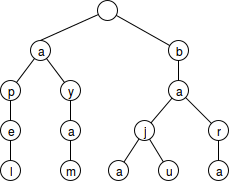
\includegraphics[scale=0.6]{pics/Contoh-StandardTrie}
    \caption{Contoh Standard Tree}
    \label{fig:contoh-standard-tree}
\end{figure}

\noindent Dari kata-kata di atas, dapat dilihat bahwa \textit{substring} `ba' paling sering muncul dibandingkan dengan yang lain yaitu muncul tiga kali.

%-----------------------------------------------------------------------------%
\subsection{Suffix Tree} \label{sec:suffix-tree}
%-----------------------------------------------------------------------------% 
\textit{Suffix tree} sering digunakan untuk pencarian \textit{sequence} yang panjang seperti \textit{genomes} untuk bidang bioinformatik. Pembentukan \textit{suffix tree} \citep{ukkonen1995line} mirip dengan pembentukan \textit{standard tree} dengan perbedaan jumlah \textit{path} yang dihasilkan dari satu \textit{string} masukan. Jika diberikan \textit{string} dengan panjang $n$, dibentuk \textit{tree} dengan cabang sebanyak $n(n-1)/2$ \textit{suffix}.  Metode ini banyak dimanfaatkan untuk mempercepat proses pencarian jika diberikan sebuah masukan \textit{query}. Jika terdapat sebuah \textit{sequence query} dengan panjang $m$, maka waktu yang dibutuhkan untuk menjalankan proses \textit{pattern matching} adalah $O(dm)$ dengan $d$ adalah ukuran alfabet. Proses pencarian dilakukan dengan menelusuri \textit{path} dari \textit{root} sesuai dengan \textit{sequence query} yang diberikan. Jika seluruh karakter dalam \textit{query} selesai dijalankan, maka proses pencarian dinyatakan berhasil. 

Sebagai contoh \textit{string} 'babaa' menghasilkan \textit{suffix tree} yang dapat dilihat pada gambar \ref{fig:contoh-suffix-tree}. Jika diberi \textit{query} 'ba' maka akan berhasil terhadap \textit{path} 'babaa' dan 'baa'.
\begin{figure}
    \centering
    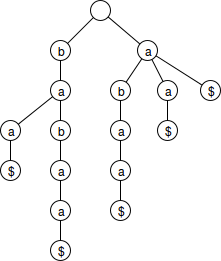
\includegraphics[scale=0.6]{pics/Contoh-SuffixTree}
    \caption{Contoh Suffix Tree}
    \label{fig:contoh-suffix-tree}
\end{figure}

\noindent Dari contoh di atas, proses pencarian dapat dijalankan dengan cepat karena seluruh \textit{suffix} telah didaftarkan ke dalam \textit{tree}. Dari \textit{query} yang ingin dicari, dapat langsung dicocokan setiap karakternya.

%
%-----------------------------------------------------------------------------%
\section{Semi-Supervised Learning}
%-----------------------------------------------------------------------------%
Dalam \textit{machine learning} terdapat dua tipe pendekatan yang umum digunakan yaitu \textit{supervised} dan \textit{unsupervised learning}. \textit{Supervised} menggunakan data berlabel sebagai data \textit{training} maupun \textit{testing}. Dari kedua data tersebut, dibentuk suatu \textit{classifier} yang dapat memenuhi segala kasus yang mungkin terjadi. Data \textit{testing} digunakan untuk menguji \textit{classifier} yang terbentuk. \textit{Unsupervised} menggunakan data yang tidak diberi label sama sekali dan berusaha untuk menemukan pola yang sama untuk suatu kumpulan data tertentu \citep{prakash2014survey}. Pendekatan lain yang merupakan kombinasi antara \textit{supervised} dan \textit{unsupervised learning} adalah \textit{semi-supervised learning}. 

\textit{Semi-supervised} adalah pendekatan \textit{machine learning} di mana informasi \textit{supervised} data diberikan tidak untuk seluruh data. Sebagian data merupakan data berlabel sementara sebagian lainnya belum memiliki label. Beberapa metode penerapan \textit{semi-supervised} adalah \textit{bootstrapping} (\textit{self training}), \textit{mixture models}, \textit{graph based methods}, \textit{co-training,} dan \textit{multiview learning}.
%(12) MITPress - Semi-Supervised Learning

%-----------------------------------------------------------------------------%
\subsection{Bootstrapping}
%-----------------------------------------------------------------------------% 
Model \textit{bootstrapping} merupakan salah satu model \textit{semi-supervised learning} yang paling umum digunakan. \textit{Bootstrapping} menggunakan data berlabel berukuran kecil dan data tidak berlabel berukuran jauh lebih besar. Proses anotasi data tidak berlabel dilakukan secara bertahap melalui sejumlah iterasi. Dari data \textit{training} berlabel, dibentuk suatu \textit{classifier} yang kemudian digunakan untuk menganotasi data tidak berlabel. Sejumlah $k$ data baru yang merupakan hasil pelabelan tersebut, dimasukkan ke dalam kelompok data berlabel. Proses tersebut dilakukan secara berulang, sehingga semakin lama iterasi jumlah data berlabel akan bertambah. 

Terdapat dua algoritma \textit{bootstrapping} yang pernah digunakan untuk proses berbasis \textit{pattern} yaitu \textit{Meta-Bootstrapping} dan \textit{Basilisk} \citep{riloff2003learning}. Keduanya digunakan untuk mengelompokkan kata ke dalam suatu kategori semantik jika diberikan korpus teks yang belum dianotasi dan sejumlah \textit{seed}. \textit{Seed} didefinisikan sebagai korpus kata yang sudah diketahui kategori semantiknya. Secara umum, proses ini akan mencari \textit{pattern} berdasarkan \textit{seed} yang diberikan. Dari \textit{pattern} yang dihasilkan dan teks yang belum dianotasi, diekstrak entitas baru dan dikelompokan berdasarkan kategori semantiknya. Kata-kata tersebut akan digabungkan ke dalam korpus pasangan kata berelasi.

%-----------------------------------------------------------------------------%
\subsection{Meta-Bootstrapping}
%-----------------------------------------------------------------------------% 
\textit{Meta-Bootstrapping} adalah salah satu variasi dari \textit{bootrapping} yang memanfaatkan \textit{pattern} dalam \textit{cycle semi-supervised}-nya. Berikut adalah beberapa proses \citep{riloff1999learning} yang dijalankan algoritma ini jika diberikan \textit{seed} berukuran kecil yang berasal dari suatu kategori semantik dan korpus yang belum dianotasi.
\begin{enumerate}
  \item Mengekstraksi \textit{pattern} secara otomatis dengan menerapkan \textit{syntactic template}.
  \item \textit{Pattern} diberi bobot berdasarkan jumlah \textit{seed} yang membentuknya.
  \item Diambil \textit{pattern} terbaik dan seluruh \textit{seed} lama yang membangun \textit{pattern} maupun \textit{seed} baru yang berhasil diesktrak oleh \textit{pattern} tersebut.
  \item Dilakukan pembobotan ulang untuk setiap \textit{pattern} menggunakan \textit{seed} lama dan baru.
\end{enumerate}

Proses di atas dinamakan \textit{mutual bootstrapping} dan setelah proses tersebut selesai, semua entitas baru hasil ekstraksi dievaluasi. Pembobotan entitas baru yang terekstrak berdasarkan jumlah \textit{pattern} yang mengekstrak kata tersebut. Lima kata terbaik diterima dan dimasukkan ke kamus (korpus) kata berelasi untuk selanjutnya diproses ulang. \textit{Pattern} terbaik berikutnya merupakan hasil ekstraksi dari \textit{seed} awal ditambah lima kata baru, sehingga \textit{pattern} untuk setiap iterasi dapat berubah. 

%-----------------------------------------------------------------------------%
\subsection{Basilisk}
%-----------------------------------------------------------------------------% 
Mirip seperti \textit{Meta-Bootstrapping}, algoritma \textit{Basilisk} \citep{thelen2002bootstrapping} juga memanfaatkan \textit{pattern} dan \textit{seed} dalam membangun korpus untuk suatu kategori semantik tertentu. Proses dapat mengekstrak lebih dari satu kategori semantik. Beberapa tahapan yang dijalankan jika diberikan korpus yang belum diantoasi dan beberapa \textit{seed} untuk setiap kategori semantik adalah sebagai berikut.
\begin{enumerate}
  \item Secara otomatis membentuk \textit{pattern} dan memberi bobot berdasarkan jumlah seed yang menghasilkan \textit{pattern}. \textit{Pattern} yang dianggap dapat mengekstrak \textit{seed} dimasukkan ke dalam \textit{pattern pool}.
  \item Untuk setiap entitas baru yang terekstraksi dari \textit{pattern}, dimasukkan ke dalam \textit{candidate word pool}. Pemberian bobot dilakukan berdasarkan jumlah \textit{pattern} yang mengekstraksi dan asosiasi kumulatif antara kata dengan \textit{seed} pada suatu kategori semantik.
  \item Lima kata terbaik diambil dan dimasukkan ke dalam kamus (korpus) yang kemudian digunakan untuk iterasi selanjutnya. 
\end{enumerate}

\textit{Basilisk} memberi bobot berdasarkan informasi kolektif dari kumpulan \textit{pattern} yang mengekstrak kata tersebut. Sementara \textit{Meta-Bootstrapping} hanya mengambil satu \textit{pattern} terbaik dan mengelompokkan seluruh kata yang terekstrak dari \textit{pattern} ke dalam kategori semantik yang sama. Dari hasil penelitian komparatif yang pernah dilakukan \citep{riloff2003learning}, didapatkan \textit{Basilisk} mengungguli performa \textit{Meta-Bootstrapping}. 


%-----------------------------------------------------------------------------%
\section{Evaluasi}
%-----------------------------------------------------------------------------%
Evaluasi dilakukan untuk mengetahui kebaikan hasil penelitian. Evaluasi dapat dilakukan dengan mengukur akurasi data yang dihasilkan. Akurasi adalah nilai perbandingan antara jumlah data yang benar dengan jumlah seluruh data \citep{manning2008introduction}. 
\begin{equation}
akurasi=\frac{jumlah\,\,data\,\,benar}{jumlah\,\,seluruh\,\,data}
\end{equation}
Selain menghitung akurasi, proses evaluasi juga menghitung nilai-nilai lainnya. Berikut ada beberapa metode dan teknik evaluasi lain yang digunakan dalam penelitian.

%-----------------------------------------------------------------------------%
\subsection{Sampling}
%-----------------------------------------------------------------------------% 
Terdapat dua kategori utama dalam \textit{sampling} yaitu \textit{probability} dan \textit{non-probability sampling}. Perbedaan utama keduanya adalah pada \textit{probability sampling}, diambil data secara acak (\textit{random}). Dalam \textit{probability sampling}, terdapat beberapa metode yang dapat digunakan seperti \textit{simple random sampling}, \textit{systematic sampling}, \textit{stratified random sampling}, dan \textit{cluster sampling} \citep{barreiro2001population}.
\begin{itemize}
  \item \textit{Simple random sampling} perlu mengetahui seluruh data yang ada dan dari data tersebut dipilih secara acak. Hal ini membuat seluruh data memiliki nilai probabilitas terpilih yang sama. 
  \item \textit{Systematic sampling} memilih setiap data ke-n untuk dijadikan \textit{sample}. 
  \item \textit{Stratified random sampling} akan mengelompokkan data ke dalam kategori berdasarkan karakteristik tertentu (strata), kemudian data diambil secara acak dari kategori yang ada. Hal ini menyebabkan hasil lebih representatif. 
  \item \textit{Cluster} sampling mirip seperti \textit{stratified sampling} namun dilakukan jika data kelompok yang ingin di-\textit{sampling} sulit berada di lokasi yang terpisah jauh.
\end{itemize}

Proses \textit{sampling} bermanfaat untuk merepresentasikan data tanpa perlu mengevaluasi seluruh data yang ada. Jika jumlah data yang ingin dievaluasi berukuran besar, proses \textit{sampling} mempercepat pengukuran. Jumlah data yang direpresentasikan oleh satu sample berdasarkan jumlah data asli. Sebagai contoh jika total data adalah 1000 dan jumlah data sample adalah 50, maka satu data \textit{sample} merepresentasikan 20 data asli.
%(Sumber: https://ecduganda.files.wordpress.com/2014/08/how-to-choose-sampling-techniques-for-evaluations.pdf)
%(optimierung.mathematik.uni-kl.de/mamaeusch/veroeffentlichungen/ver_texte/sampling_en.pdf)

%-----------------------------------------------------------------------------%
\subsection{Precision dan Recall}
%-----------------------------------------------------------------------------% 
Teknik yang umum digunakan untuk mengevaluasi suatu ekstraksi adalah \textit{precision} dan \textit{recall}. \textit{Precision} adalah nilai yang menyatakan jumlah dokumen benar dan berhasil diambil dibandingkan dengan seluruh jumlah dokumen yang terambil. \textit{Recall} adalah nilai yang menyatakan jumlah dokumen benar dan berhasil diambil dibandingkan dengan jumlah seluruh dokumen yang benar. Semakin banyak dokumen yang diambil maka nilai \textit{recall} akan meningkat sementara nilai \textit{precision} cenderung menurun. 

%-----------------------------------------------------------------------------%
\subsection{Kappa}
%-----------------------------------------------------------------------------%  
Nilai kappa ($\kappa$) merepresentasikan tingkat persetujuan antar anotator. Kappa digunakan pada penelitian yang menggunakan bantuan anotator untuk memberi penilaian secara manual. Peniliaian didapatkan menggunakan rumus \ref{kappa}.

\begin{equation}
\label{kappa}
\kappa=\frac{P(A)-P(E)}{1-P(E)}
\end{equation}

\begin{itemize}
  \item $P(A)$ adalah proporsi penilaian yang setuju (\textit{agreement})
  \item $P(E)$ adalah proporsi penilaian yang kebetulan
\end{itemize}

\noindent \cite{landis1977measurement} mendefiniskan tingkat persetujuan berdasarkan nilai Kappa yang diperoleh. 
\begin{table}
  \centering
    \caption{Skala pengukuran Kappa}
    \label{table:skalaKappa}
    \begin{tabular}{|c|c|}
      \hline
      Statistik Kappa & Tingkat persetujuan \\ \hline
      < 0.00 & \textit{Poor} \\ \hline
      0.00 - 0.20 & \textit{Slight} \\ \hline
      0.21 - 0.40 & \textit{Fair} \\ \hline
      0.41 - 0.60 & \textit{Moderate} \\ \hline
      0.61 - 0.80 & \textit{Substantial} \\ \hline
      0.81 - 1.00 & \textit{Almost Perfect} \\ \hline
    \end{tabular}
\end{table}

Beberapa variasi perhitungan untuk Kappa adalah Cohen's Kappa dan Fleiss' Kappa. Cohen's Kappa digunakan untuk mengukur tingkat persetujuan antar dua anotator. Jika diberikan data dengan $n$ label dan $m_ij$ merepresentasikan jumlah data yang diberi label $i$ oleh anotator pertama dan label $j$ oleh anotator kedua, maka proses perhitungan $P(A)$ dan $P(E)$ untuk Cohen's Kappa adalah sebagai berikut.
\[ P(A)=\frac{\sum_{k=1}^{n} m_kk}{total\,\,data} \]
\[ P(E)=\frac{\sum_{k=1}^{n} ( \sum_{j=1}^{n} m_kj . \sum_{i=1}^{n} m_ik ) }{total\,\,data} \]

Fleiss' Kappa mengukur tingkat persetujuan antar sekelompok anotator berjumlah lebih dari dua. Jika diberikan $N$ data dengan $n$ anotator di mana setiap data diantosi ke dalam salah satu dari $k$ kategori dan $n_ij$ merepresentasikan total anotator yang memberi data $i$ ke label $j$, proses perhitungan $P(A)$ dan $P(E)$ untuk Fleiss' Kappa adalah sebagai berikut.
\[ P(A)=\frac{1}{N}\sum_{i=1}^{N}P_i \:\:\:\:\:dengan\:\:\:\:\: P_i=\frac{1}{n(n-1)}[(\sum_{j=1}^{k}n^2_ij)-(n)] \]

%-----------------------------------------------------------------------------%
\subsection{Spearman's Rho}
%-----------------------------------------------------------------------------% 
\textit{Spearman's rank correlation coefficient} adalah nilai koefisien korelasi antar \textit{ranking} dua parameter. Nilai \textit{Spearman correlation} sama dengan nilai \textit{Pearson correlation} antar dua paramter yang telah di-\textit{ranking}. \textit{Pearson correlation}  menggambarkan nilai linear antara dua parameter. \textit{Spearman correlation} berkisar antara $-1$ hingga $+1$.

Spearman's rho adalah nilai Pearson Correlation Coefficient antar dua variabel yang telah di-\textit{ranking}. Untuk mendapatkan nilai koefisien ($r_s$), menggunakan rumus berikut.
\begin{equation}
r_s = \rho_{rg_X,rg_Y} = \frac{cov(rg_X,rg_Y)}{\sigma_{rg_X}\sigma_{rg_Y}}
\end{equation}
\begin{itemize}
  \item $\rho$ adalah \textit{Pearson correlation coefficent} yang diaplikasikan pada variabel \textit{ranking}
  \item $cov(rg_X,rg_Y)$ adalah nilai \textit{covariance} antar variabel \textit{ranking}
  \item $\sigma_{rg_X}$ dan $\sigma_{rg_Y}$ adalah nilai standard deviasi variabel \textit{ranking}
\end{itemize}

\noindent Jika seluruh \textit{ranking} berbeda, proses komputasi dapat dilakukan menggunakan rumus berikut.
\begin{equation}
r_s = 1-\frac{6 \Sigma d_i^2}{n(n^2-1)}
\end{equation}
\begin{itemize}
  \item $d_i = rg(X_i)-rg(Y_i)$ adalah selisih antara dua \textit{ranking}
  \item $n$ adalah jumlah observasi
\end{itemize}


% %-----------------------------------------------------------------------------%
% %-----------------------------------------------------------------------------%
% \section{Pointwise Mutual Information}
% %-----------------------------------------------------------------------------%
% \textit{Pointwise Mutual Information} (PMI) adalah pengukuran nilai asosiasi antar variabel. Dalam bidang \textit{information theory}, PMI dapat dimanfaatkan untuk menghitung asosiasi kemunculan dua buah kata. Jika diberikan dua buah kata $x$ dan $y$, maka nilai PMI kata tersebut dalam suatu dokumen dapat dihitung menggunakan rumus berikut. 
% \[ pmi(x;y)=log\frac{p(x,y)}{(x)p(y)}=log\frac{p(x|y)}{p(x)}=log\frac{p(y|x)}{p(y)} \] dengan $p(x)=\frac{f(x)}{N}$
% \[ pmi(x;y)=log\frac{f(x)N}{f(x)f(y)} \]
% \begin{itemize}
%   \item $p(x)$ adalah probabilitas kemunculan kata $x$ dalam korpus
%   \item $f(x)$ adalah frekuensi kemunculan kata $x$ dalam korpus
%   \item $N$ adalah toatal seluruh kata dalam korpus
% \end{itemize}
% Pengukuran ini bersifat simetris, sehingga $p(x;y)=p(y;x)$. Nilai PMI dapat merupakan bilangan POSitif maupun negatif. Jika nilai PMI adalah nol (0), berarti kedua variabel saling \textit{independent}.

% %-----------------------------------------------------------------------------%
% \subsection{Skip PMI}
% %-----------------------------------------------------------------------------% 
% PMI umumnya hanya menggunakan model \textit{bigram} atau \textit{trigram}. Model ini hanya melihat hubungan kata yang berdampingan. Sebagai contoh ingin diketahui PMI untuk \textit{bigram} 'hong kong', 'sepak bola', dan 'amerika serikat'. Pada penelitian ini dilakukan modifikasi yaitu membuat model \textit{skip-gram} PMI. Kita menghitung nilai PMI antar dua kata yang dipisahkan dengan $n$ di antaranya. 
